\documentclass{labreport}

% UTF-8 support for Romanian diacritics in code listings
\lstset{style=python,
  literate={ă}{{\v{a}}}1
           {â}{{\^{a}}}1
           {î}{{\^{i}}}1
           {ș}{{\c{s}}}1
           {ț}{{\c{t}}}1
           {Ă}{{\v{A}}}1
           {Â}{{\^{A}}}1
           {Î}{{\^{I}}}1
           {Ș}{{\c{S}}}1
           {Ț}{{\c{T}}}1
}

\begin{document}

% ---------------------------------------------------------
% 1. TITLE PAGE
% ---------------------------------------------------------
\labtitle{1}{Laboratory Work 1: Concurrency in Practice}{Ilie Covali}{gr. FAF-243}{asist. univ. Cristofor Fistic}

\tableofcontents
\newpage

% ---------------------------------------------------------
% 2. OBJECTIVE AND SYSTEM SPECIFICATION
% ---------------------------------------------------------
\section{Objective and Requirements}

\subsection{Laboratory Objective}
The objective of this laboratory work is to investigate real-world multithreaded concurrency in systems programming, measuring how thread counts and workload partitioning strategies influence execution time, parallel speed-up, and peak memory utilization. Key goals include:
\begin{enumerate}
    \item Observing CPU-bound workload scaling across physical cores and logical processors.
    \item Identifying parallel speed-up saturation points and context-switching penalties.
    \item Demonstrating race conditions and non-deterministic memory corruption in unsynchronized concurrent updates.
    \item Quantifying the performance overhead of mutual exclusion (locks) compared to thread-local aggregation.
\end{enumerate}

\subsection{Hardware and Runtime Environment}
To ensure true OS-level thread concurrency without the Global Interpreter Lock (GIL), the implementation uses the newly released \textbf{free-threaded CPython 3.13} runtime, managed via the \texttt{uv} package and virtual environment manager.

\begin{table}[H]
\centering
\caption{Hardware and Environment Specifications}
\label{tab:hardware}
\begin{tabular}{ll}
\toprule
\textbf{Component} & \textbf{Specification} \\
\midrule
CPU Model & AMD Ryzen 3 4300U with Radeon Graphics \\
Architecture & x86\_64 (Zen 2) \\
Physical Cores & 4 \\
Logical Processors & 4 (1 thread per core, SMT disabled) \\
RAM & 19.4 GB DDR4 \\
Storage Subsystem & WDC PC SN530 NVMe SSD (256 GB) \\
Operating System & CachyOS Linux (Kernel 7.2.9-2-cachyos) \\
Programming Language & Python 3.13.16+freethreaded (Clang 23.1.3 build) \\
GIL Status & Disabled (\texttt{sys.\_is\_gil\_enabled() == False}) \\
Environment Tool & \texttt{uv} 0.12+ \\
\bottomrule
\end{tabular}
\end{table}

\subsection{Dataset Generation}
The input dataset consists of a text file \texttt{numbers.txt} containing exactly $50\,000\,000$ uniformly distributed pseudo-random integers in the range $[-1\,000\,000, 1\,000\,000]$, formatted with one number per line. The file size is approximately $352.33\text{ MB}$.
\begin{equation}
\text{Total} = \text{Count}(\text{negative}) + \text{Count}(\text{positive}) + \text{Count}(\text{zero}) = 50\,000\,000
\end{equation}
Every implemented task must satisfy this strict conservation invariant.

\newpage

% ---------------------------------------------------------
% 3. TASK 1a: COUNTING WITH THREADS
% ---------------------------------------------------------
\section{Task 1a: Direct File Partitioning and Multithreaded Sign Counting}

\subsection{Methodology and Boundary Handling}
Task 1a evaluates parallel file reading and counting across thread configurations $T \in \{1, 2, 4, 8, 16, 32, 64\}$. Reading the entire file on a single thread or pre-loading the text into RAM is prohibited. The file of size $S$ bytes is partitioned into $T$ disjoint nominal byte intervals:
\begin{equation}
\text{Range}_t = \left[ \left\lfloor \frac{t \cdot S}{T} \right\rfloor, \left\lfloor \frac{(t + 1) \cdot S}{T} \right\rfloor \right), \quad t \in \{0, 1, \dots, T - 1\}
\end{equation}

Because nominal byte offsets arbitrarily split text lines, a boundary reconciliation algorithm is implemented:
\begin{itemize}
    \item \textbf{Initial Seek:} Thread $t > 0$ seeks to byte offset $\text{start}_t - 1$ and inspects the preceding character. If the preceding character is a newline (\texttt{\textbackslash n}), the thread begins parsing immediately at $\text{start}_t$. If it is not a newline, the thread discards the remainder of the fractional line via \texttt{readline()} and begins parsing from the next complete line.
    \item \textbf{Termination Boundary:} Threads $t < T - 1$ continue reading lines until their byte counter satisfies $\text{curr\_pos} \ge \text{end}_t$. The fractional line spanning across $\text{end}_t$ is fully consumed by thread $t$, ensuring that the subsequent thread $t + 1$ (which discards up to that line's newline) will neither skip nor duplicate any record.
    \item \textbf{Tail Processing:} Thread $T - 1$ reads continuously until EOF.
\end{itemize}

\subsection{Experimental Results}
The benchmark was executed with 2 separate runs per thread configuration using isolated subprocesses to capture exact peak resident set size (Peak RSS).

\begin{table}[H]
\centering
\small
\caption{Task 1a Benchmark Results ($50\,000\,000$ integers, NVMe SSD)}
\label{tab:task1a_results}
\begin{tabular}{ccccccc}
\toprule
\textbf{Threads} & \textbf{Run 1 (ms)} & \textbf{Run 2 (ms)} & \textbf{Avg Time (ms)} & \textbf{Speed-up} & \textbf{Peak RAM (MB)} & \textbf{Total Counted} \\
\midrule
1  & 6921.9 & 6870.8 & 6896.3 & 1.00$\times$ & 29.6 & 50 000 000 \\
2  & 5021.7 & 5051.0 & 5036.3 & 1.37$\times$ & 31.4 & 50 000 000 \\
4  & 2773.6 & 2804.5 & 2789.0 & 2.47$\times$ & 35.5 & 50 000 000 \\
8  & 2716.1 & 2644.2 & 2680.1 & 2.57$\times$ & 44.0 & 50 000 000 \\
16 & 2719.3 & 2791.0 & 2755.1 & 2.50$\times$ & 60.2 & 50 000 000 \\
32 & 2704.6 & 2717.6 & 2711.1 & 2.54$\times$ & 52.0 & 50 000 000 \\
64 & 2689.1 & 2776.1 & 2732.6 & 2.52$\times$ & 46.0 & 50 000 000 \\
\bottomrule
\end{tabular}
\end{table}

\textbf{Correctness verification:} Across all thread configurations (1 through 64), every single trial produced identical sign totals:
\begin{equation}
\text{Negative} = 25\,002\,492, \quad \text{Positive} = 24\,997\,491, \quad \text{Zero} = 17, \quad \text{Total} = 50\,000\,000
\end{equation}
This confirms that the boundary-seeking logic operates with zero omission and zero duplication.

\begin{figure}[H]
\centering
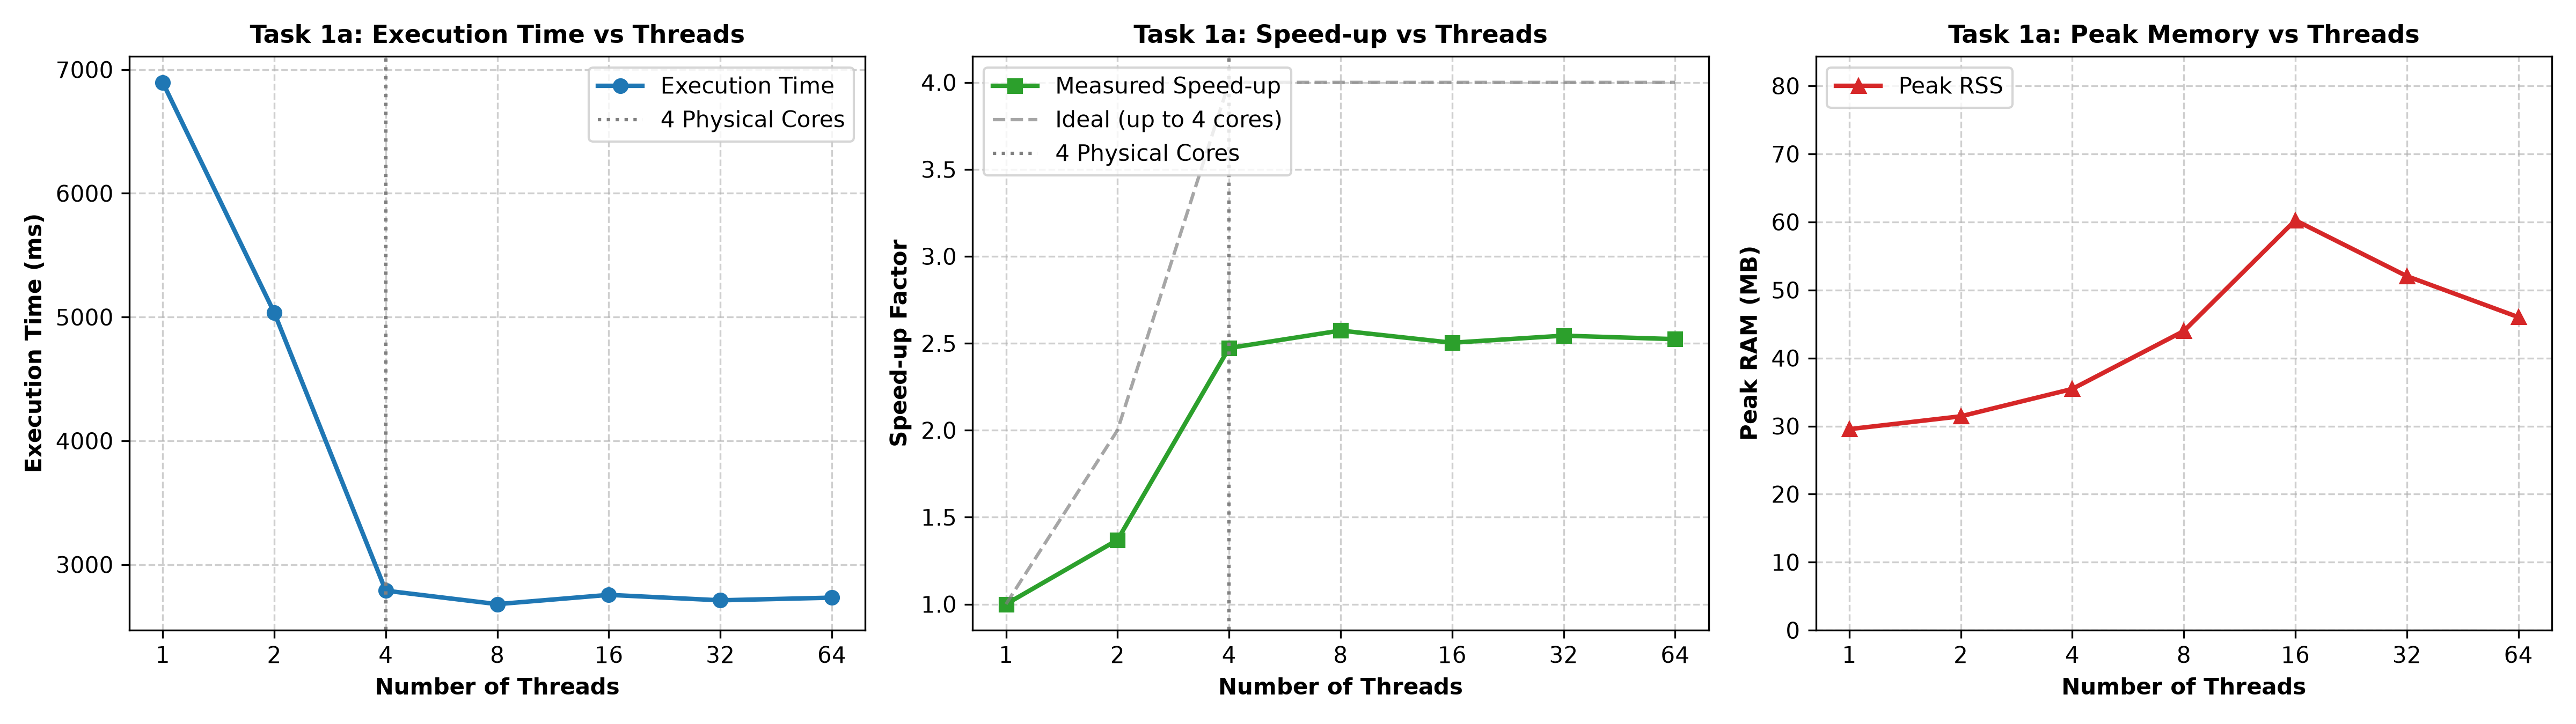
\includegraphics[width=\textwidth]{images/fig1_task1a.png}
\caption{Task 1a: Execution time, speed-up, and peak memory versus thread count.}
\label{fig:task1a}
\end{figure}

\subsection{Discussion and Analysis}
\begin{enumerate}
    \item \textbf{Scaling Behavior:} Execution time drops dramatically from $6896.3\text{ ms}$ on 1 thread to $2789.0\text{ ms}$ on 4 threads, yielding a $2.47\times$ speed-up. Because the test CPU possesses 4 physical execution cores without SMT, scaling scales directly up to 4 threads.
    \item \textbf{Plateau Beyond 4 Threads:} For 8, 16, 32, and 64 threads, execution time plateaus at $\approx 2.7\text{ seconds}$ ($2.50\times - 2.57\times$ speed-up). Over-subscribing 4 physical cores with 64 OS threads introduces operating system scheduler overhead and register context switching, which prevents any further speed gains.
    \item \textbf{Memory Invariance:} Peak RAM remains modest between $29.6\text{ MB}$ and $60.2\text{ MB}$. Because each thread streams lines directly from disk using small internal file buffers, memory usage is decoupled from the dataset size ($352\text{ MB}$).
\end{enumerate}

\newpage

% ---------------------------------------------------------
% 4. TASK 1b: THREE WAYS TO COUNT
% ---------------------------------------------------------
\section{Task 1b: Three Synchronization Strategies for Sign Counting}

\subsection{Experimental Setup}
In Task 1b, all $50\,000\,000$ integers are preloaded into a contiguous in-memory 32-bit signed integer buffer using Python's native \texttt{array.array('i')}. The array occupies $190.73\text{ MB}$ of contiguous memory.

With thread count matched to the machine's 4 logical execution processors ($T = 4$), the elements are partitioned into 4 uniform slices of $12\,500\,000$ integers. The signs are counted under three distinct synchronization paradigms:
\begin{enumerate}
    \item \textbf{Version 1 (Unsynchronized Shared Counters):} All 4 threads concurrently execute in-place increments (\texttt{shared.neg += 1}, \texttt{shared.pos += 1}, \texttt{shared.zero += 1}) without locks or atomics.
    \item \textbf{Version 2 (Lock-Protected Counters):} Every counter update is enclosed within a mutual exclusion lock (\texttt{threading.Lock()}).
    \item \textbf{Version 3 (Thread-Local Counters):} Each thread independently counts signs in local CPU registers/variables. Totals are summed into a global accumulator only after all threads finish.
\end{enumerate}

\subsection{Experimental Results}
As mandated by the laboratory specification, Version 1 was executed three consecutive times to observe race condition non-determinism.

\begin{table}[H]
\centering
\small
\caption{Task 1b Benchmark Results ($T = 4$ threads, $50\,000\,000$ in-memory integers)}
\label{tab:task1b_results}
\begin{tabular}{lcccccc}
\toprule
\textbf{Synchronization Version} & \textbf{Run 1 (ms)} & \textbf{Run 2 (ms)} & \textbf{Run 3 (ms)} & \textbf{Avg Time (ms)} & \textbf{Counted} & \textbf{Correct?} \\
\midrule
Version 1 (Unsynchronized) & 9977.1 & 10015.0 & 10017.6 & 10003.2 & 38 458 125 & \textbf{No} (Lost 23\%) \\
Version 2 (Lock-Protected)  & 18818.6 & --- & --- & 18818.6 & 50 000 000 & \textbf{Yes} \\
Version 3 (Thread-Local)    & 2386.4 & --- & --- & \textbf{2386.4} & 50 000 000 & \textbf{Yes} \\
\bottomrule
\end{tabular}
\end{table}

\begin{figure}[H]
\centering
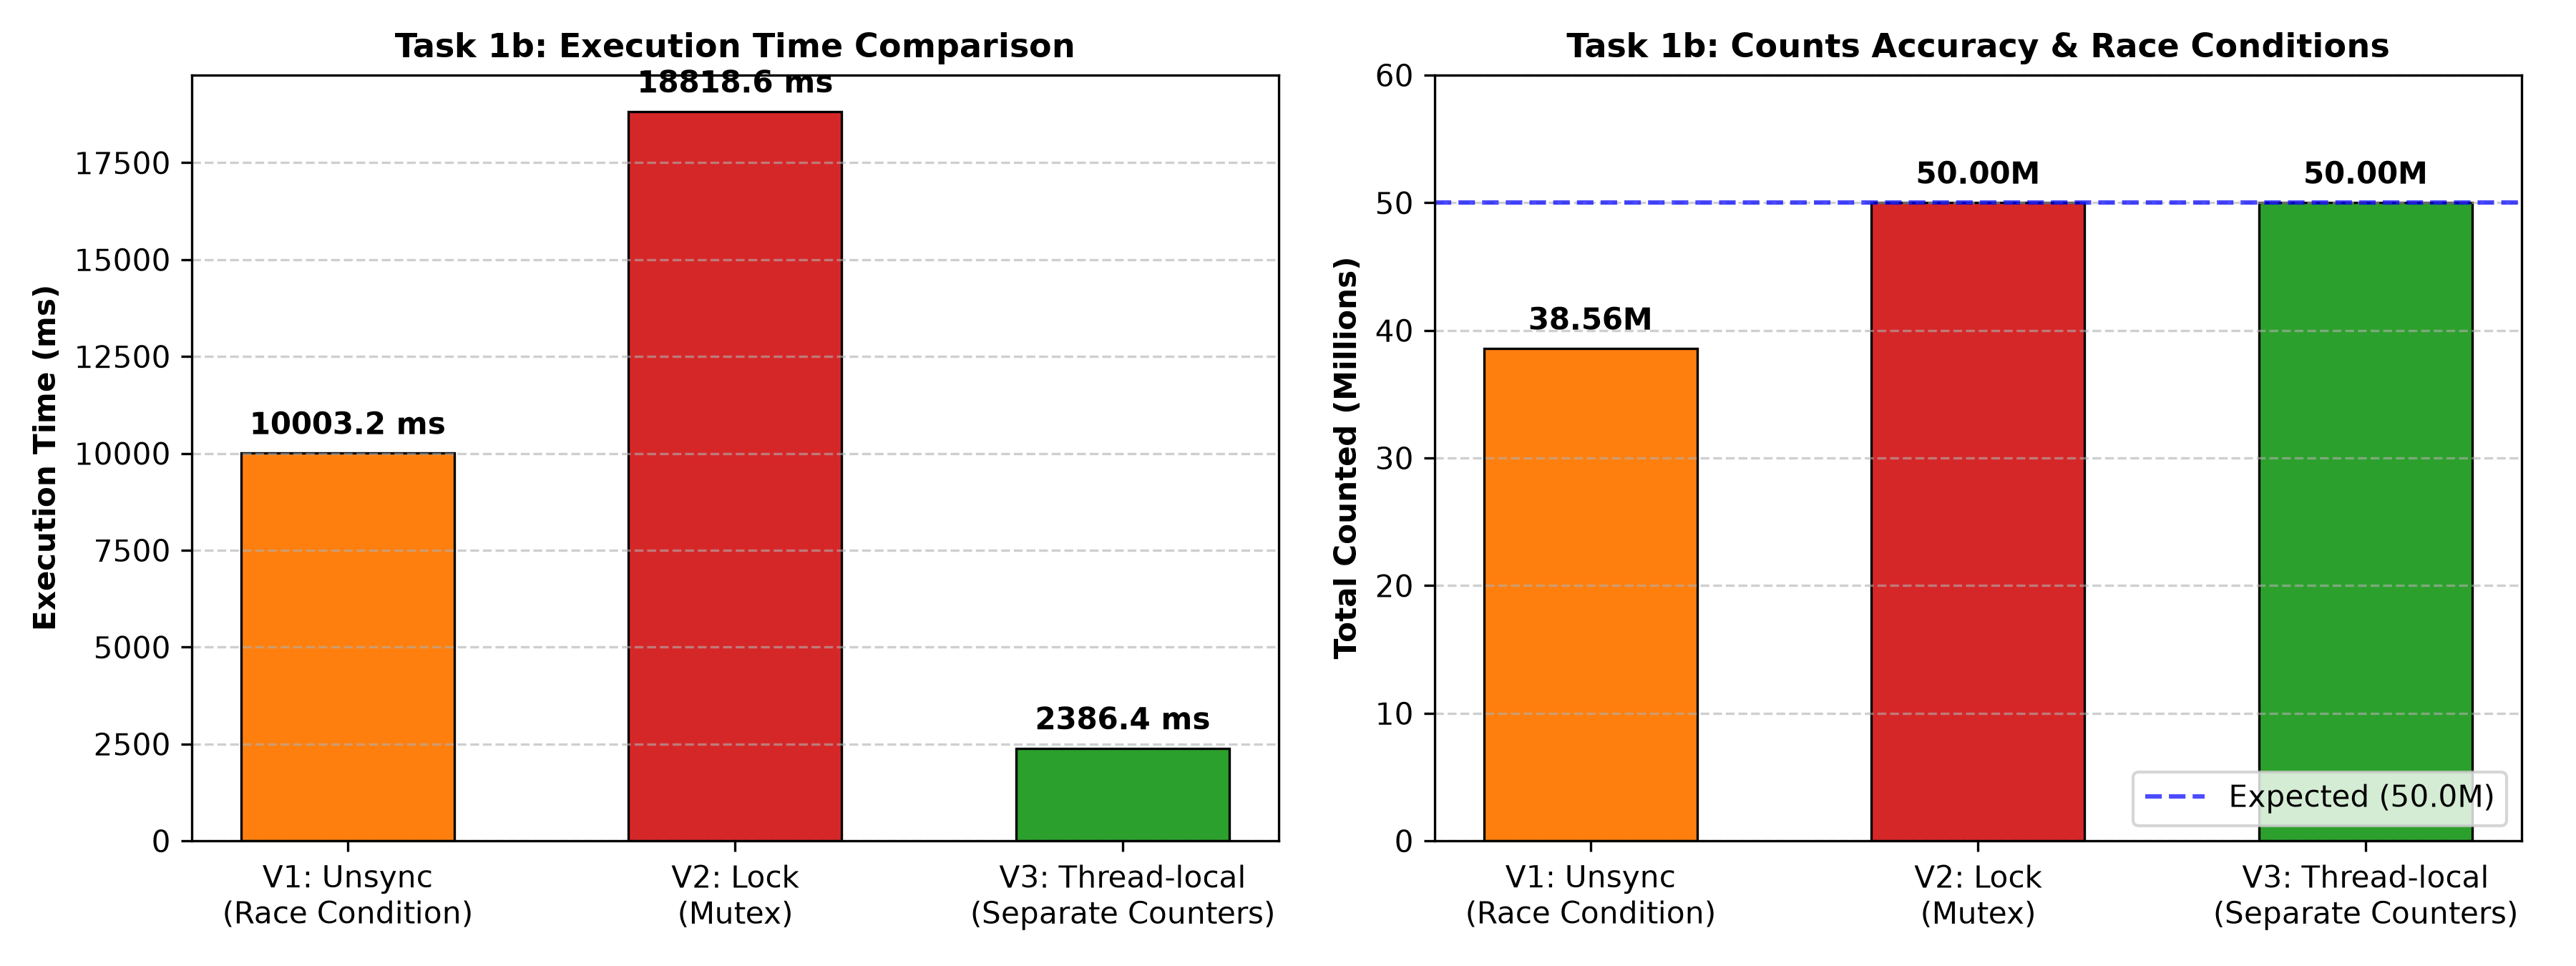
\includegraphics[width=\textwidth]{images/fig2_task1b.png}
\caption{Task 1b: Execution time and total numbers counted across the three synchronization approaches.}
\label{fig:task1b}
\end{figure}

\subsection{Discussion and Analysis}
\begin{enumerate}
    \item \textbf{Demonstration of Race Conditions in Free-Threaded Python:}
    In standard CPython, the Global Interpreter Lock serialize bytecode execution, masking many race conditions. In free-threaded Python 3.13t with GIL disabled, \texttt{shared.neg += 1} expands to discrete load-increment-store instructions executed concurrently across 4 hardware cores. Multiple cores simultaneously read identical values, overwrite each other's increments, and lose over $11.5\text{ million}$ updates ($\approx 23\%$ data loss). Furthermore, the three runs of Version 1 produced distinct counts ($38\,458\,125$, $38\,995\,000$, and $38\,237\,826$), proving non-deterministic execution.
    \item \textbf{Overhead of Lock Contention:}
    Version 2 guarantees correctness ($50\,000\,000$ counted), but requires $18\,818.6\text{ ms}$---a massive \textbf{7.89$\times$ slowdown} compared to Version 3 ($2386.4\text{ ms}$). Because all 4 cores attempt to acquire the identical mutex $50\,000\,000$ times, cache lines holding the lock bounce between CPU L1/L2 caches, causing extreme bus contention and thread stalls.
    \item \textbf{Dominance of Thread-Local Aggregation:}
    Version 3 is the fastest and most efficient paradigm. Threads operate strictly on private stack variables residing in fast L1 cache with zero synchronization overhead. A single $O(T)$ summation at the end yields exact correctness in only $2.38\text{ seconds}$.
\end{enumerate}

\newpage

% ---------------------------------------------------------
% 5. UNFINISHED SECTIONS AS REQUESTED
% ---------------------------------------------------------
\section{Task 1c: Producer and Consumers Pipeline}
\textit{[Note: This section is left unfinished as requested by the user.]}

\vspace{1cm}

\section{Task 2: Many Files on Slow Storage}
\textit{[Note: This section is left unfinished as requested by the user.]}

\vspace{1cm}

\section{Control Questions and Conclusion}
\textit{[Note: This section is left unfinished as requested by the user.]}

\end{document}
